\section{Executable shape editing and evaluation}
\label{sec:method}
Figure~\ref{fig:mechanical-flow} links a realistic four-to-six mounting-hole request to the actual final 3B patch, edited solid and numerical fields. The source solid is an illustration of the program input, not a model input image.
\begin{figure*}[t]
\centering
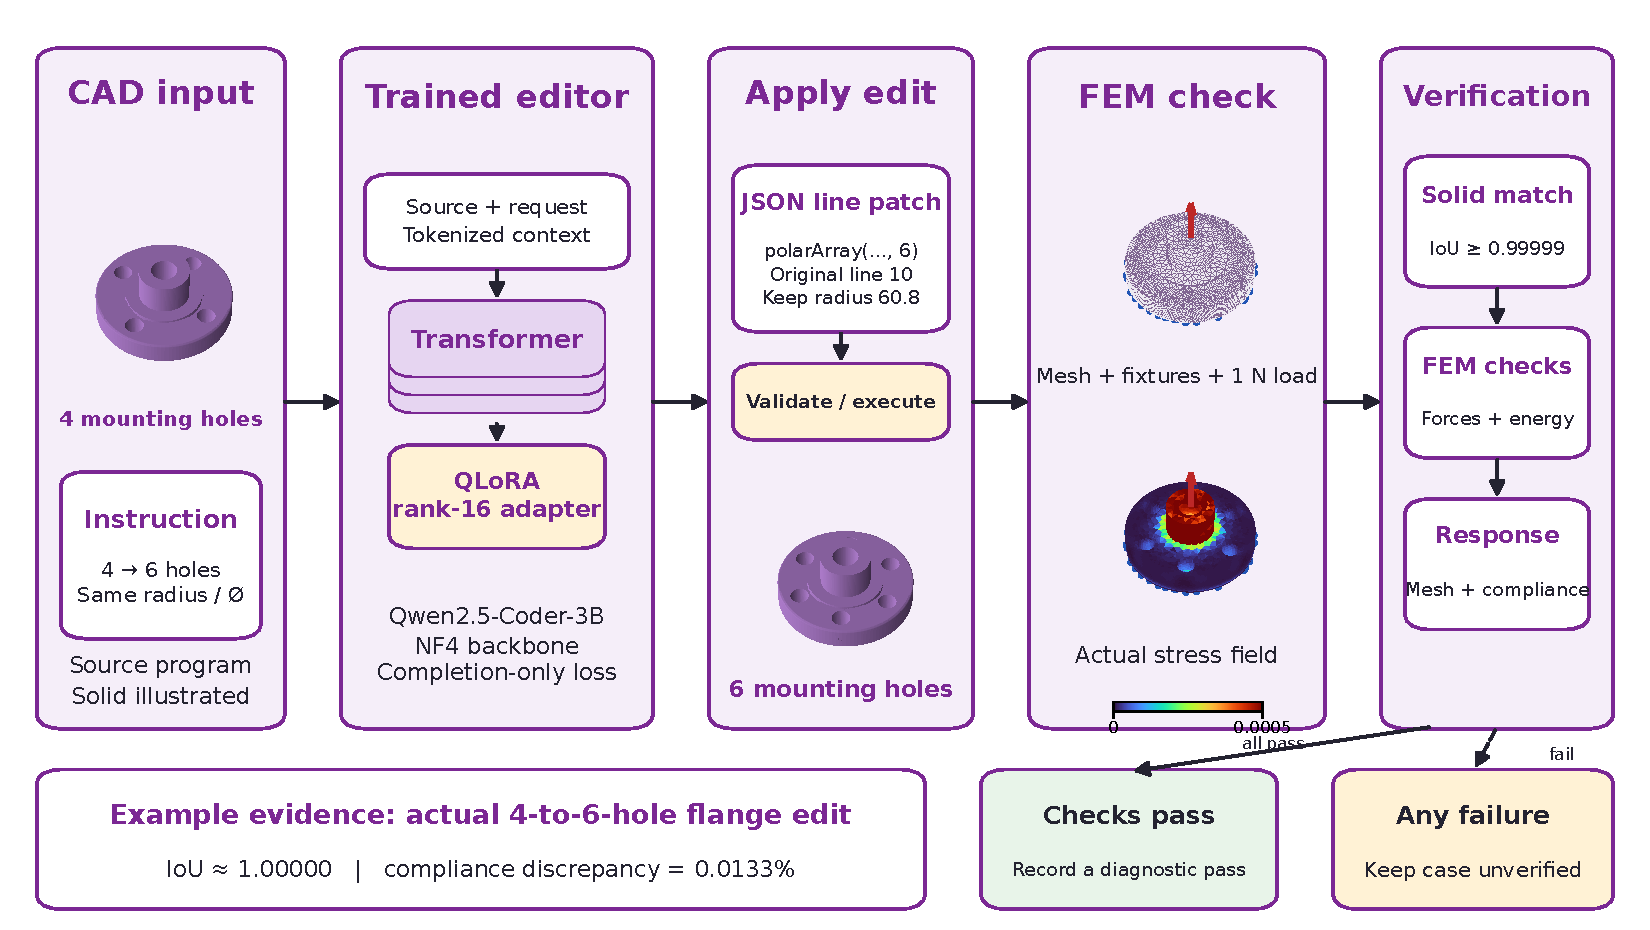
\includegraphics[width=0.98\textwidth]{figures/cad-fem-illustrated-architecture.pdf}
\caption{\textbf{Instruction-guided executable 3D editing.} Native CAD and text condition the trained editor. Validated patches produce the edited solid; views, solid comparison and optional FEM inspect that result. The shown flange is an actual final 3B prediction changing four holes to six at the same diameter and bolt-circle radius. Its saved tetrahedral mesh, fixture (blue), load (red) and von Mises field use a declared synthetic 1 N test; stress is clipped at p95 in MPa. FEM is an external diagnostic, not training supervision. Failed stages remain unverified.}
\label{fig:mechanical-flow}
\end{figure*}
\subsection{Model and patch contract}
Given source representation $C$ and instruction $u$, the model predicts patch $p$ and the executor returns $\hat C=\mathcal E(C,p)$. Each operation specifies a zero-based original line index, deletion count and replacement-line list. Operations must be typed, ordered, non-overlapping and in bounds. All coordinates address the original source. CadQuery syntax or native command-schema validation follows patch application.

We fine-tune Qwen2.5-Coder-3B-Instruct~\cite{hui2024qwen25coder} with NF4 double quantization and completion-only QLoRA~\cite{hu2022lora}. For supervised pairs $(C,u,p^\star)$, only answer tokens contribute to
\begin{equation}
\mathcal L_{\rm edit}=-\sum_{t\in\mathrm{answer}}\log P_{\theta,\phi}(p_t^\star\mid C,u,p_{<t}^\star),
\end{equation}
where $\theta$ denotes frozen base weights and $\phi$ the adapters. No image features, FEM loss, verifier reward or test-based checkpoint choice enters training. The architecture in Fig.~\ref{fig:mechanical-models} documents the native-representation branches.

\subsection{Execution and solid agreement}
The appropriate CAD backend builds a boundary-representation solid $\hat B$. Successful execution requires valid geometry, at least one solid and positive volume. The CadQuery executor permits a restricted set of imports and builtins, rejects private-attribute access and file I/O, and applies a 45-second per-case subprocess budget. This is defense in depth, not a general Python sandbox. Unsupported constructs and operational failures remain separate outcomes.

For target $B^\star$, volumetric intersection-over-union is
\begin{equation}
J_{\rm vol}=\frac{V(\hat B\cap B^\star)}{V(\hat B)+V(B^\star)-V(\hat B\cap B^\star)}.
\end{equation}
We use local broad and strict thresholds of 0.95 and 0.99999, respectively. Exact normalized program/sequence and patch matches are complementary diagnostics. None certifies engineering tolerances, preserved constraints or manufacturing suitability.

\subsection{Common-camera view and edit measurements}
We derive front, top, right and isometric views from each solid. The linked SVG sheets are CAD-derived views, not independently predicted images or production blueprints. For the focused visual audit, tetrahedral FEM is unnecessary: tessellated boundary surfaces are rasterized into binary orthographic silhouettes $S_v(B)$.

For each case and view $v$, source, target and available predictions share projection axes, image scale and center. Bounds use their union; no individual shape is recentered. We render 512- and 1,024-pixel square images with 0.3\,mm tessellation tolerance. This is a diagnostic camera contract, including available output bounds, rather than a predictor-independent camera benchmark.

For source solid $B$, define reference and predicted changes as
\begin{equation}
\Delta_v^\star=S_v(B)\oplus S_v(B^\star),\quad
\hat\Delta_v=S_v(B)\oplus S_v(\hat B),
\end{equation}
where $\oplus$ is binary exclusive-or. We report both silhouette IoU and edit-mask IoU $J_{\rm edit,v}=\operatorname{IoU}(\Delta_v^\star,\hat\Delta_v)$. Empty unions are undefined and excluded from the edit mean; nonempty unintended changes are retained. This exposes differences in the changed region, but cannot measure occluded/internal features or instruction semantics. Very small change masks are sensitive to rasterization; we disclose their effect rather than infer feature correctness from a scalar average.

\subsection{Conditional mechanical response audit}
FEM is applied only with an explicit physical contract. The illustrated BenchCAD scenarios assume mm/N/MPa units, $E=210{,}000$ MPa, $\nu=0.3$, a fixed lower 5\,\% surface band and an upper-band resultant of 1 N. These are declared test conditions, not recovered properties or operating loads. Native CAD-Editor examples lack established physical scale and are not assigned such results.

First-order tetrahedra solve small-strain 3D isotropic elasticity with $K_e=V_eB_e^TDB_e$ and fixed-degree elimination. We check finite solutions, anchored components, residuals, force/moment balance and $2U=\mathbf f^T\mathbf u$ to normalized error below $10^{-6}$. Refinement targets at most 5\,\% compliance change; a local response diagnostic compares predicted and target compliance within 10\,\%. This complements solid agreement and does not certify stress convergence or safety. Full contracts and saved fields appear in Appendix~\ref{sec:mechanical-fem}.
